\section{Results and Discussion} \label{results}

\subsection{Single-Precision RT-CC}\label{result:precision}

For the last 35 years (and updated most recently in 2019),the IEEE 754
standard\cite{IEEE-754-2019} has defined ``interchange and arithmetic formats
and methods for binary and decimal floating-point arithmetic in computer
programming environments,'' {\em i.e.}\ the representation and mathematical
operations of single- and double-precision numbers, among others.  In this
standard, each floating-point number is stored with three components: a sign, a
significand/coefficient, and an exponent.  For single precision, the 23 explicit
bits of the significand (plus an implicit bit for normal numbers) yields
$\log_{10}(2^{24}) \approx 7.22$ decimal digits, whereas double precision
yields $\log_{10}(2^{53}) \approx 15.95$ decimal digits.  As mentioned in
section~\ref{intro}, the development of quantum chemical methods that take
advantage of the efficiency of single- and mixed-precision arithmetic --- both
in storage and in computing time --- have seen considerable advances in recent
years.  For size-extensive properties, such as the total electronic energy,
Ufimtsev and Mart\' inez\cite{Ufimtsev2008,Ufimtsev2008quantum} demonstrated that
purely single-precision arthimetic and storage quickly becomes inadequate as the
size of the molecular system increases.  Similar observations were reported by
Asadchev and Gordon\cite{Asadchev2012} in their mixed- and high-precision
implementation of the Rys quadrature for the evaluation of two-electron
repulsion integrals, and by Tornai and co-workers in their development of a
high-performance, dynamic integral-evaluation program.\cite{Tornai2019}
Pokhilko, Epifanovsky, and Krylov\cite{Pokhilko2018} also reported a novel
single- and mixed-precision implementation of CC and equation-of-motion CC
methods in 2018, in which solution iterations of the relevant CC equations in
single precision were adequate for most applications, and a limited number of
``cleanup'' iterations in double-precision could recover higher accuracy.  Thus,
for such cases, a mixed-precision approach wherein some steps of the quantum
chemical calculation are carried out in single precision and others in higher
precision becomes essential.  

In this work we focus on simulations of linear UV/vis absorption spectra using
the approach described earlier.  If single-precision arithmetic is adequate, the
computational cost can be reduced to nearly half for both small and large
systems, and the error will not accumulate as the system size increases,
assuming neither the dipole moment nor the relevant electronic-excitation
domains are extensive.  To test this assumption, we computed the time-dependent
dipole moments of the water molecule at a series time points from a
double-precision RT-CCSD/cc-pVDZ calculation and corrupted the data by adding
random noise at several magnitude cutoffs.  In this initial test, we carried out
the time propagation for 300 a.u.\ using a Gaussian envelope with a field
strength ${\cal E} = 0.01$ a.u., center $\nu = 0.05$ a.u., width $\sigma = 0.01$
a.u., and a time step $h = 0.01$ a.u.

As shown in Fig.~\ref{fig:sp-noise}, the spectrum begins to deviate from
the original dipole trajectory only with random noise added starting at a magnitude
of $10^{-5}$ and greater.  In such cases, the spectra manifest the appearance of
the noise typically in the low-frequency region, as can be seen in the upper two
spectra between 0-5 eV.  Smaller noise cutoffs yield spectra that are
indistinguishable from their noise-free counterpart.  This is consistent with
the expectation based on the IEEE definition of floating-point arithmetic,
namely that single-precision can retain accuracy to roughly $10^{-7}$. 
\begin{figure}
    \centering
    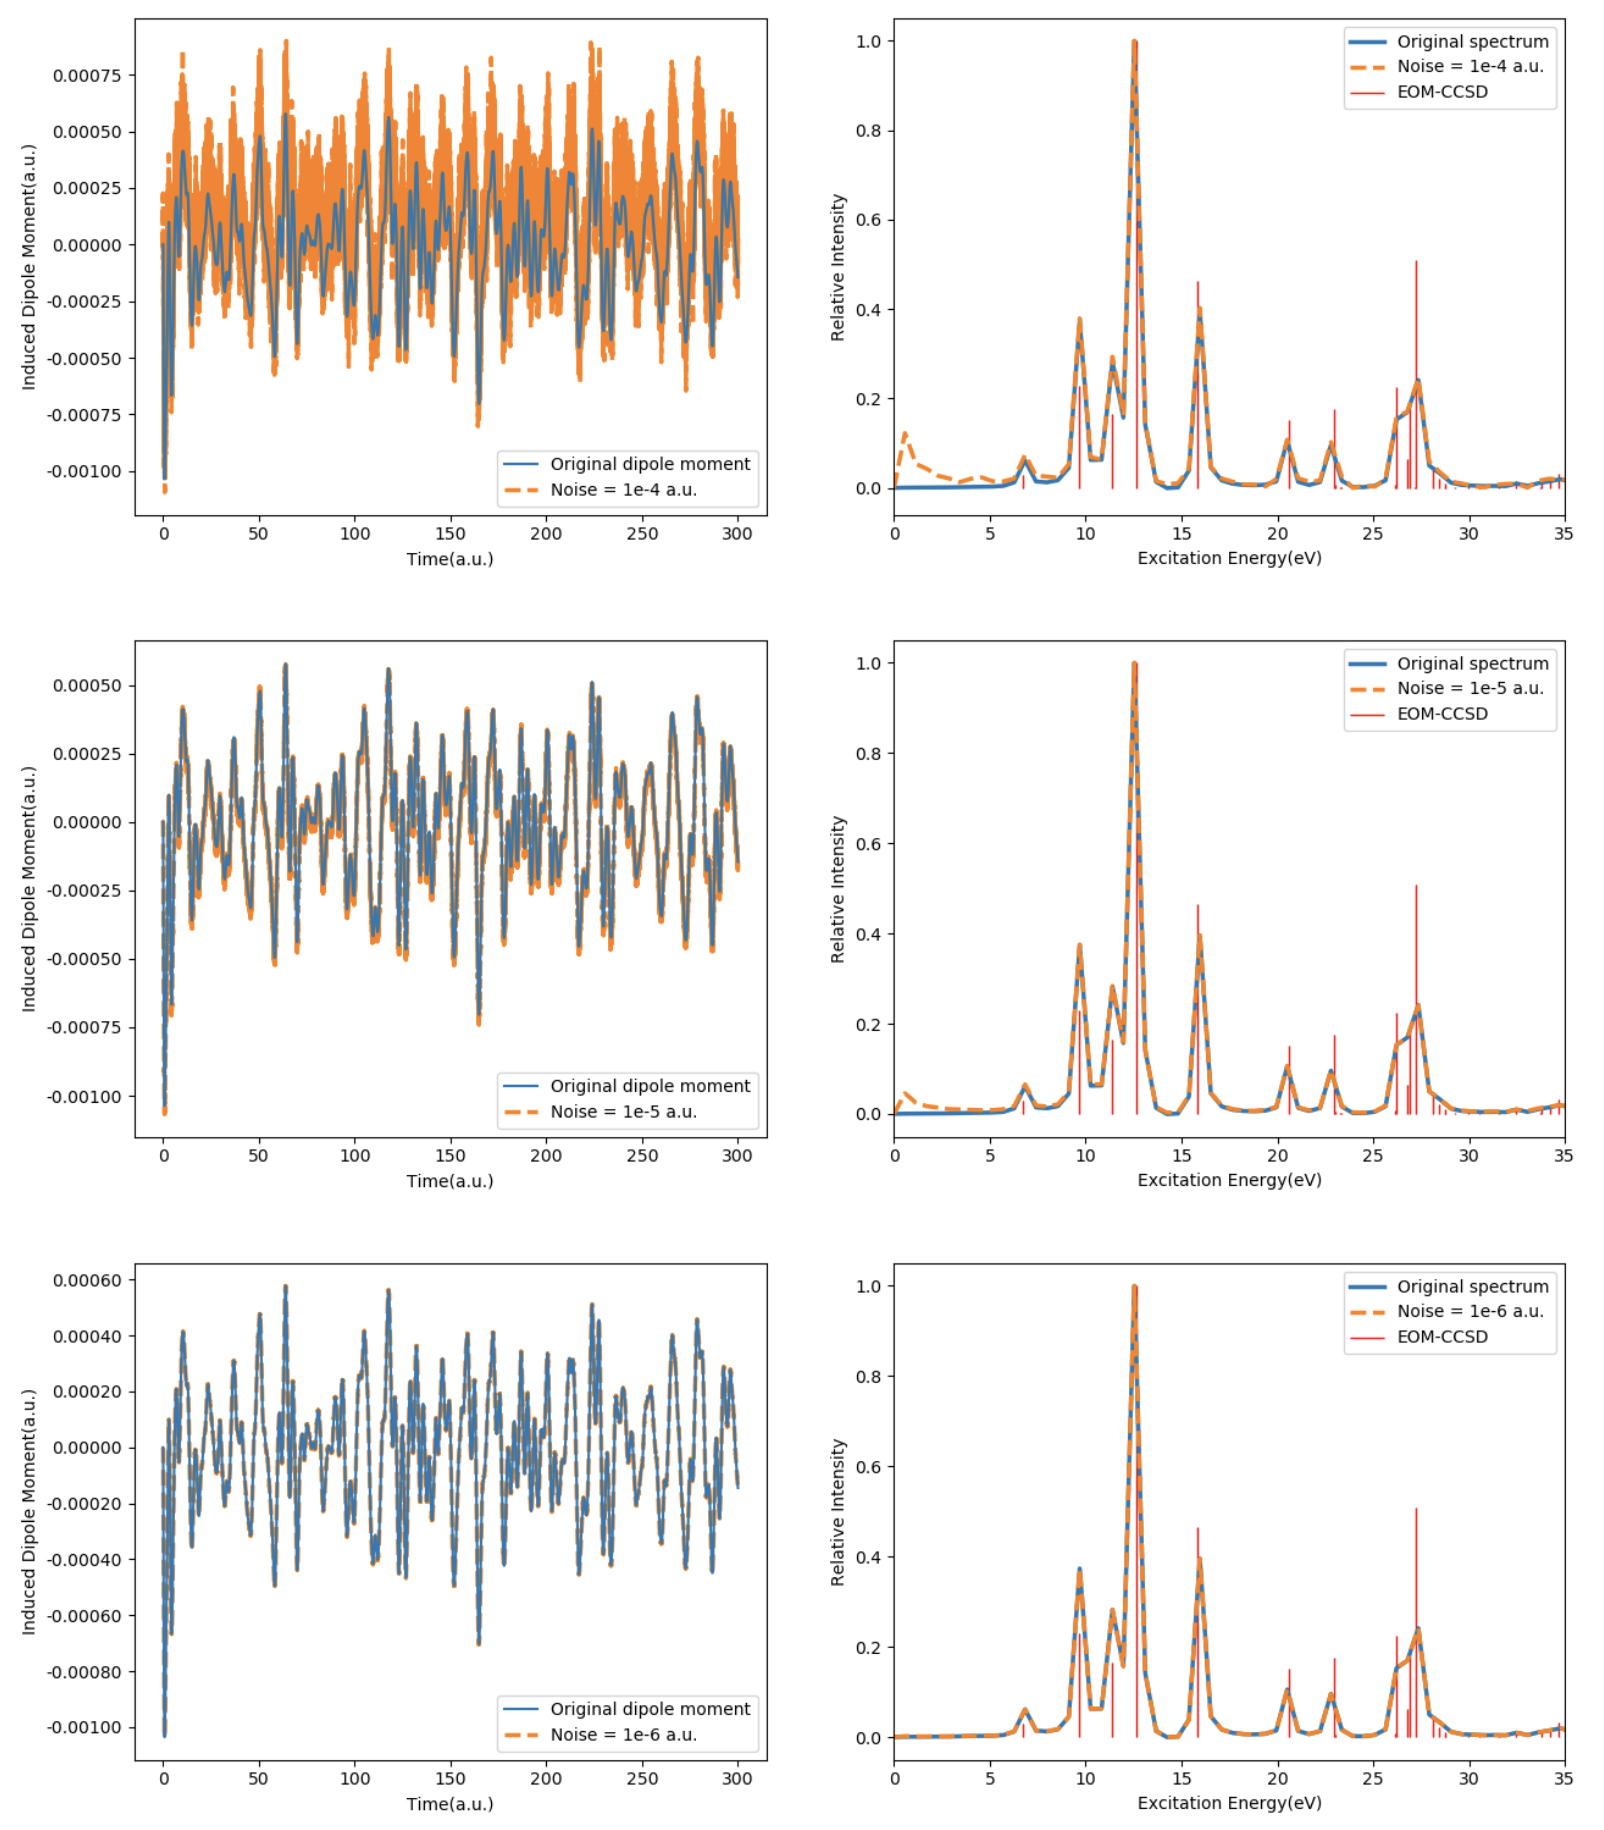
\includegraphics[angle=0, scale=0.6]{ch3/Figs/1-5.png}
    \caption{RT-CCSD/cc-pVDZ time-dependent induced electric dipole moments (left-hand
column) for a water molecule in the presence of an external electric field and
the corresponding linear absorption spectrum (right-hand column) with and
without random noise of varying magnitudes. Corresponding EOM-CCSD/cc-pVDZ 
transitions are included as stick-spectra for comparison.}
    \label{fig:sp-noise}
\end{figure}

To compare the double-precision and single-precision arithmetic directly, we
calculated the RT-CCSD/cc-pVDZ dipole trajectories and corresponding linear
absorption spectra shown in Fig.~\ref{fig:sp-spectrum} using both representations for the series of (H$_2$O)$_n$
clusters with $n=1-4$. For these simulations, the explicit integration was
carried out using the Runge-Kutta 4th order integrator (RK4) with a step size
$h=0.01$ a.u.  The external field was chosen to be a Gaussian envelope defined
in Eq.~(\ref{eq:field}) with ${\cal E} = 0.01$ a.u., $\nu=0.05$ a.u., and
$\sigma=0.01$ a.u. (a narrow pulse). The results are aligned with the numerical
experiments above, with no discernible difference in the spectra after lowering
the arithmetic precision to single-precision. All the spectra are also compared
with EOM-CCSD/cc-pVDZ calculations: we include 40 EOM-CC roots in each of the
spectra, all of which are well-aligned with the associated RT-CC peaks. From this perspective,
the computation time and the required size of memory can both be reduced by
ca.\ a factor of two for the calculation of the spectra, as previously observed
for electronic energies and other components of quantum chemical
calculations.\cite{Ufimtsev2008,Ufimtsev2008quantum,Asadchev2012,Tornai2019,Pokhilko2018}
We note, however, that single-precision arithmetic may not be practical for certain numerically sensitive calculations,
\textit{e.g.}, using higher-order numerical differentiation to extract linear and nonlinear response functions as reported
by Ding \textit{et al.}\cite{Ding2013}
(In addition, we note that these spectra are not intended to reproduce vapor-phase experimental
measurements, only to test the validity of the single-precision arithmetic
approximation.  Thus, any transitions appearing above the physical ionization
limit are not physically realistic and are merely an artifact of the use of a
finite basis set without representation of continuum states.)

\begin{figure}
     \centering
     \begin{subfigure}{0.475\textwidth}
         \centering
         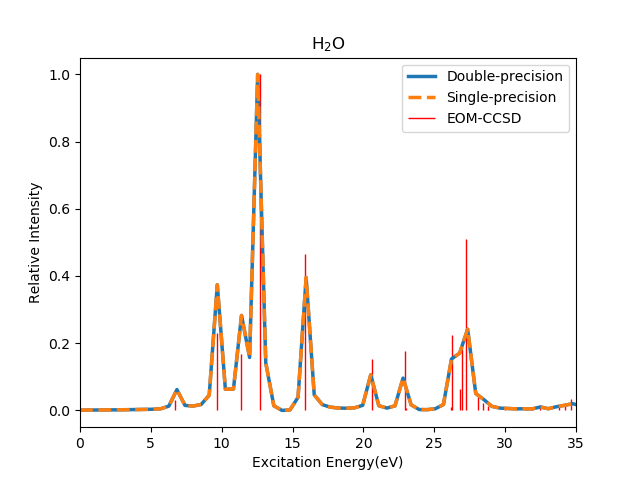
\includegraphics[width=\textwidth]{ch3/Figs/1-1.png}
         \label{fig:sp-monomer}
     \end{subfigure}
     \hfill
     \begin{subfigure}{0.475\textwidth}
         \centering
         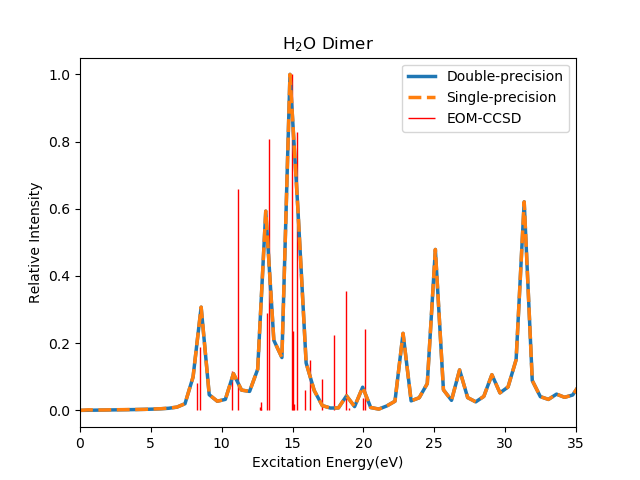
\includegraphics[width=\textwidth]{ch3/Figs/1-2.png}
         \label{fig:sp-dimer}
     \end{subfigure}
     \vfill
     \begin{subfigure}{0.475\textwidth}
         \centering
         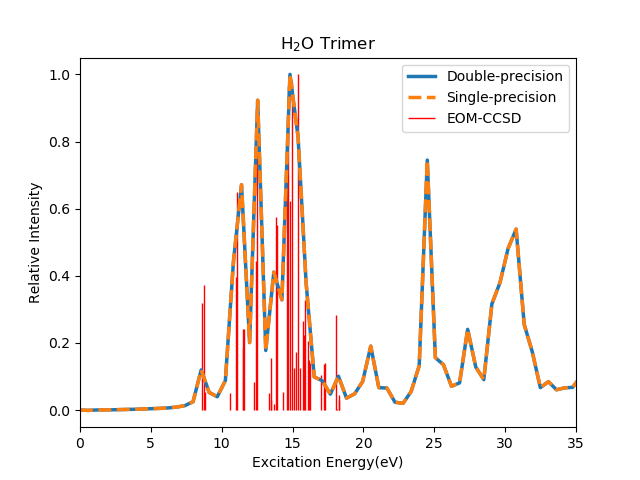
\includegraphics[width=\textwidth]{ch3/Figs/1-3.png}
         \label{fig:sp-trimer}
     \end{subfigure}
     \hfill
     \begin{subfigure}{0.475\textwidth}
         \centering
         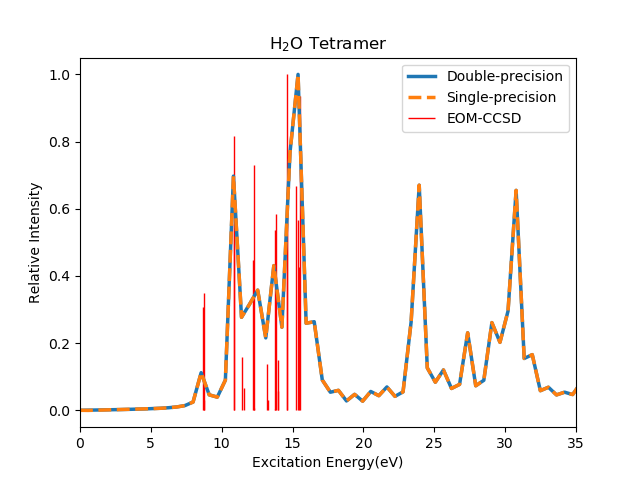
\includegraphics[width=\textwidth]{ch3/Figs/1-4.png}
         \label{fig:sp-tetramer}
     \end{subfigure}
     \caption{Linear UV/vis absorption spectra of (H$_{2}$O)$_n$ clusters for
$n=1-4$ calculated at the RT-CCSD/cc-pVDZ level of theory in both double- and
single-precision arithmetic. Time propagation was carried out for 300 a.u. in
the presence of a weak electric field represented by a narrow Gaussian pulse.
Corresponding EOM-CCSD/cc-pVDZ transitions are included as stick-spectra for
comparison.}
     \label{fig:sp-spectrum}
\end{figure}

Inspired by many parallel implementations of CC methods for distributed memory
architectures on CPUs\cite{Olson2007, Solomonik2014, Janowski2007,
Anisimov2014}, corresponding GPU implementations have become desirable in order
to take advantage of heterogenous artchitectures on modern high-performance
computing systems.  While early GPU hardware was designed for accelerating image
processing with an emphasis on mostly single- or low-precision floating point
operations for quick memory access when higher accuracy is not required, over
the past several years, GPUs have been more extensively used for scientific
research.  In addition to the development of GPUs with robust performance for
double-precision arithmetic, numerous software toolkits have also emerged such
as the Computer Unified Device Architecture (CUDA),\cite{cuda} the Open
Computing Language (OpenCL),\cite{Stone2010} and a variety machine-learning
packages that support GPUs such as TensorFlow,\cite{tensorflow2015}
PyTorch,\cite{Paszke2019} and others, all of which lower the barriers to a wide
range of scientific applications that can take advantage of modern GPU
performance.  We note that, even though the performance of double-precision
calculations on GPUs is already relatively robust, single-precision arithmetic
is still preferable if it provides neglible errors relative to double-precision
results due to the substantial improvement in computational speed and memory
usage.  

For the RT-CC methods explored in this work, we have therefore developed a
GPU-capable implementation within the PyCC code using the PyTorch
package\cite{Paszke2019} based on the conventional CPU version described in
section~\ref{comp}.  In the PyCC implementation, all one-electron quantities
such as the Fock matrix (including the external field), $\hat{T}_1$, and
$\hat{T}_2$ amplitudes are loaded onto the GPU at the beginning of either each
iteration of the time-independent wave function or each computation of the
residuals in Eqs.~(\ref{Eq:derivT}) and (\ref{Eq:derivL}) during the RT-CC
propagation.  As each term in the CC equations is evaluated, the necessary
subblock of the two-electron repulsion integrals is loaded onto the GPU, and the
required tensor contraction is carried out using the usual {\tt opt\_einsum}
function.  Other two- and four-index intermediates formed from the
similarity-transformed Hamiltonian (\textit{e.g.}, the $W_{mbej}$ or $W_{amef}$
intermediates), are retained on the GPU as they are created for later use in the
same iteration/time-step, and deleted once the current residual is complete.
The advantage of this approach is that it provides straightforward access to
local GPU hardware without significant modification of the NumPy-based
tensor-contraction code already in place.  Of course, this Python-based
implementation does not represent the full performance of a production-level
code and is necessarily limited in terms of the size of the molecular system it
can treat, but it does provide a valuable estimate of the minimum expected
speed-up one can obtain for a more highly optimized alogrithm.

Table~\ref{tab:gpu-cpu} provides a comparison of RT-CCSD/cc-pVDZ timings for
double-precision (dp) and single-precision (sp) on CPUs and GPUs for our set of
example water clusters, using the same Gaussian envelope parameters are for
previous computations.  The first three columns report the number of seconds
required for each time step of the RT-CC simulation averaged over a 300 a.u.
propagation (\textit{i.e.}, for a step size of $h=0.01$ a.u., averaged over
30,000 time steps).  As the size of the molecular system increases from monomer
to tetramer, the computational cost per iteration for a CPU-dp calculation
increases by approximately a factor of ca.\ $4^{4.85}$, whereas for a GPU-dp
calculation, the increase is a factor of ca.\ $4^{3.18}$, and for a GPU-sp
calculation, this falls to $4^{2.88}$.  While these are clearly less than the
formal ${\cal O}(4^6)$ scaling expected from CCSD, all of these implementations
would eventually reach that limit for larger systems, because the CPU/GPU and
dp/sp improvements only affect the prefactor, and not the exponent.
Nevertheless, the use of the GPU coupled with single-precision arithmetic
clearly offers substantial advantages.  This improvement is also clearly seen in
the data reported in the final two columns of Table~\ref{tab:gpu-cpu}, where the
single-precision code yields roughly the expected factor of two speed-up over
its double-precision counterpart (with both calculations taking place on the
GPU), and the GPU offers up to a factor of 14 speed-up over the CPU when both
operate in double-precision (or better when the GPU operates in single-precision
mode).  Larger molecular systems should offer even greater improvement, with the
proviso that the memory limits of the GPU will eventually produce a performance
pleateu.
\begin{table} 
    \centering
        \caption{Performance comparison of conventional RT-CC/cc-pVDZ calculations
for water clusters using double-precision on the CPU (CPU-dp), double-precision
on the GPU (GPU-dp), and single-precision on the GPU (GPU-dp). Timings (first
three columns) are given in seconds as per-iteration averages over a 300 a.u.
propagation wth $h=0.01$ a.u.  The final two columns are speed-ups,
\textit{i.e.} ratios of timings for each case.}
    \begin{tabular}{c|ccccc}
       \textrm{Water Cluster} & $t_\textrm{CPU-dp}$ &  $t_\textrm{GPU-dp}$ &
$t_\textrm{GPU-sp}$ & $\frac{t_\textrm{CPU-dp}}{t_\textrm{GPU-dp}}$ &
$\frac{t_\textrm{GPU-dp}}{t_\textrm{GPU-sp}}$\\ \hline
       \textrm{Monomer} & 0.17217 & 0.14330 & 0.13253 & 1.2015 & 1.0813\\ 
       \textrm{Dimer} & 3.4705 & 0.60738 & 0.40496 & 5.7139 & 1.4999\\
       \textrm{Trimer} & 32.729 & 3.4910 & 1.7264 & 9.3752 & 2.0221 \\
       \textrm{Tetramer} & 167.43 & 11.727 & 7.2215 & 14.277 & 1.6239\\     
    \end{tabular}
    \label{tab:gpu-cpu}
\end{table}
        
\subsection{Comparison of Numerical Integrators for RT-CC} \label{result:integrator}

As discussed in section~\ref{theory}, the family of Runge-Kutta methods is the
most widely used class of numerical integrators for IVPs such as the TDSE, not
only because their implementation is straightforward --- \textit{e.g.}, for
RT-CC methods they are easily adapted to accept function vectors taken from the
left- and right-hand wave function residuals in Eqs.~(\ref{Eq:derivT}) and
(\ref{Eq:derivL}) --- but also because of their relatively robust performance
for a range of applications.  The classic Runge-Kutta 4th order integrator
(RK4), for example, is one of the most commonly used algorithms for scientific
problems because it averages each time step into four simple stages and yields a
small truncation error of order $h^{5}$, where $h$ is the step size,
\begin{equation}\label{eq:rk4truncation}
y_{n+1} = y_{n} + \frac{1}{6}(k_{1}+2k_{2}+2k_{3}+k_{4}) + \textit{O}(h^{5}).
\end{equation}

Such explicit integrators typically yield stable propagations of real-time
methods, provided sufficient care is taken in choosing the step size, which is
critical not only for the integration to be numerically stable, accurate, and
efficient, but also cost effective: larger step sizes reduce the computational
expense of the simulation, but they can also result in failure of the
propagation due to a non-convergent time series.  Rather than running sets of
numerical experiments to find the largest, reasonable step size that can provide
accurate results for every application, adaptive integrators\cite{Press1992}
were designed to balance the required stability with the least computational
cost by exerting algorithmic control over step size  within the existing process of
explicit integrators.  For example, Fehlberg\cite{Fehlberg1968} discovered that,
by carrying out six function evaluations per time step and using different
combinations of the six resulting intermediates to formulate a fifth-order
solution and a fourth-order solution, a fourth-order method can be derived with
step size control.  In 1990, Cash and Karp\cite{Cash1990} found another
combination of Fehlberg's coefficients that yields an even more efficient
method,
\begin{equation}\label{eq:ck-k}
\begin{aligned}
k_{1} &= f(t_{n}, y_{n})\\
k_{2} &= f\left(t_{n}+\frac{1}{5}h, y_{n}+\frac{1}{5}k_{1}h\right)\\
k_{3} &= f\left(t_{n}+\frac{3}{10}h,
y_{n}+h\left(\frac{3}{40}k_{1}+\frac{9}{40}k_{2}\right)\right)\\
k_{4} &= f\left(t_{n}+h,
y_{n}+h\left(\frac{3}{10}k_{1}+\frac{9}{10}k_{2}+\frac{6}{5}k_{3}\right)\right)\\
k_{5} &= f\left(t_{n}+\frac{3}{5}h,
y_{n}+h\left(\frac{-11}{54}k_{1}+\frac{5}{2}k_{2}-\frac{70}{27}k_{3}+\frac{35}{27}k_{4}\right)\right)\\
k_{6} &= f\left(t_{n}+\frac{7}{8}h,
y_{n}+h\left(\frac{1631}{55296}k_{1}+\frac{175}{512}k_{2}-\frac{575}{13824}k_{3}+\frac{44275}{110592}k_{4}+\frac{253}{4096}k_{5}\right)\right),
\end{aligned}
\end{equation}
with the resulting coupled time steps being,
\begin{equation}\label{eq:ck-y}
\begin{aligned}
y_{1} &=
y_{n}+h\left(\frac{37}{378}k_{1}+\frac{250}{621}k_{3}+\frac{125}{594}k_{4}+\frac{512}{1771}k_{6}\right)\\
y_{2} &=
y_{n}+h\left(\frac{2825}{27648}k_{1}+\frac{18575}{48384}k_{3}+\frac{13525}{55296}k_{4}+\frac{277}{14336}k_{5}+\frac{1}{4}k_{6}\right)
\end{aligned}
\end{equation}
where $y_{1}$ is a fourth-order solution embedded with $y_{2}$, which is a
fifth-order solution. Therefore, with $\Delta=|y_{2}-y_{1}|$ taken to be an
error estimate for the current time step of order $h^{5}$, a desired accuracy of
$\epsilon$ yields a formula for adjusting the step-size on the fly,
\textit{viz.},
\begin{equation}\label{eq:ck-h}
\frac{h_{new}}{h}=\left(\frac{\epsilon}{\Delta}\right)^{1/5}.
\end{equation}
Thus, if $\Delta$ is smaller than $\epsilon$, $h$ will be increased for the next
step, but if $\Delta$ is larger than $\epsilon$, $h$ will be reduced and the
current step must be repeated until the required accuracy is reached.
Furthermore, if $h$ is reduced and used for the current step again, the error
will have an implicit scaling of $h$, and the exponent in Eq.~(\ref{eq:ck-h})
must be shifted from $\frac{1}{5}$ to $\frac{1}{4}$. The size control of final
step is given as,
\begin{equation}\label{eq:ck-h-final}
\begin{aligned}
h_{new} &= 0.84 h \left(\frac{\epsilon}{\Delta}\right)^{1/5}   \hspace{0.5cm}&
\textrm{for} \hspace{0.1cm}|\Delta| \leq \epsilon \\
h_{new} &= 0.84 h \left(\frac{\epsilon}{\Delta}\right)^{1/4}   \hspace{0.5cm}& 
\textrm{for} \hspace{0.1cm}|\Delta| > \epsilon 
\end{aligned}
\end{equation}
where the coefficient $0.84$ is a ``safety factor'' because the error
estimates are not exact.  Thus, the computational cost of the adaptive
integrator is optimized under a predetermined desired accuracy. If the values at
consecutive time steps change rapidly, a small step size will naturally be used;
if the values vary only slightly, larger step sizes will be sufficient for a
stable propagation. 

In our RT-CC calculations, the time-dependent cluster amplitudes change rapidly
when the external field is on at the beginning of the simulation and gradually
stabilize after the field is turned off.  With this in mind, we tested the
adaptive Cash-Karp (CK) integrator described above for the RT-CCSD simulation
of the absorption spectrum of a single water molecule using the same external
field as in the calculations in section \ref{result:precision}. Additionally,
with the results shown in section \ref{result:precision}, all the calculations
are run in single-precision for the efficiency. 

Fig.~\ref{fig:ck-step} reports the variation in the step size at each iteration
of the propagation using an initial step size of $h=0.01$ a.u.  From
Eq.~(\ref{eq:field}), if $t=0.01$ a.u.\ the field strength is only $3.35\times
10^{-6}$ a.u., and the local error $\Delta$, is expected to be smaller than
$\epsilon$ according to Eq.~(\ref{eq:ck-h-final}), leading to an increase in
$h$ to 0.015 a.u.  At the second time step when $t=0.025$ a.u., the
corresponding field strength is $4.39\times 10^{-4}$ a.u., which gets closer to
its peak of 0.01 a.u.  At this point in the simulation, $\Delta$ is large, and
the CK algorithm automatically reduces the step size to $h=0.012$ a.u.  At the
third and fourth time steps, $h$ slightly increases to 0.014 a.u., because,
even though the field is still on, $h=0.012$ a.u. is small enough to keep
$\Delta$ smaller than $\epsilon$. After the fifth time step, $h$ is increased
to 0.018 a.u. and further 0.027 a.u. when $t=0.064 ~\textrm{to}~ 0.082$ a.u.,
because, during this point in the propagation, the field strength has already
begun to decrease due to the brevity of the pulse.  When the propagation
reaches $t=0.109$ a.u., the magnitude of the field strength falls back to
$10^{-10}$, $\Delta$ is small when $h=0.027$ a.u.\ is tested, and thus $h$
increases to 0.032 a.u.\ at the seventh time step and 0.057 a.u.\ at the eighth
time step. Starting from the ninth time step when $t=0.198$ a.u., although the
external field is essentially zero for the remainder of the propagation, the
algorithm still converges to a step size of $h=0.02$ a.u. due to the continued
oscillation of the amplitudes instigated by the pulse. Since the step size varies 
throughout the propagation, the dipole moments are not calculated at equally 
spaced time points, typical Fourier transform will not work, instead, we pre-process 
our data by interpolating the data points to an evenly spaced grid. Ultimately, after a 300
a.u.\ propagation, the adaptive CK integrator yields an overall speedup of 1.32
relative to the explicit RK4 integrator, yet, as shown in
Fig.~\ref{fig:ck-results}, the final absorption spectra obtained from each
algorithm exhibit no significant differences.  Thus, adaptive integrators such
as the CK algorithm can provide an automated approach to systematically
optimizing the step size depending on the system.

\begin{figure}
    \centering
    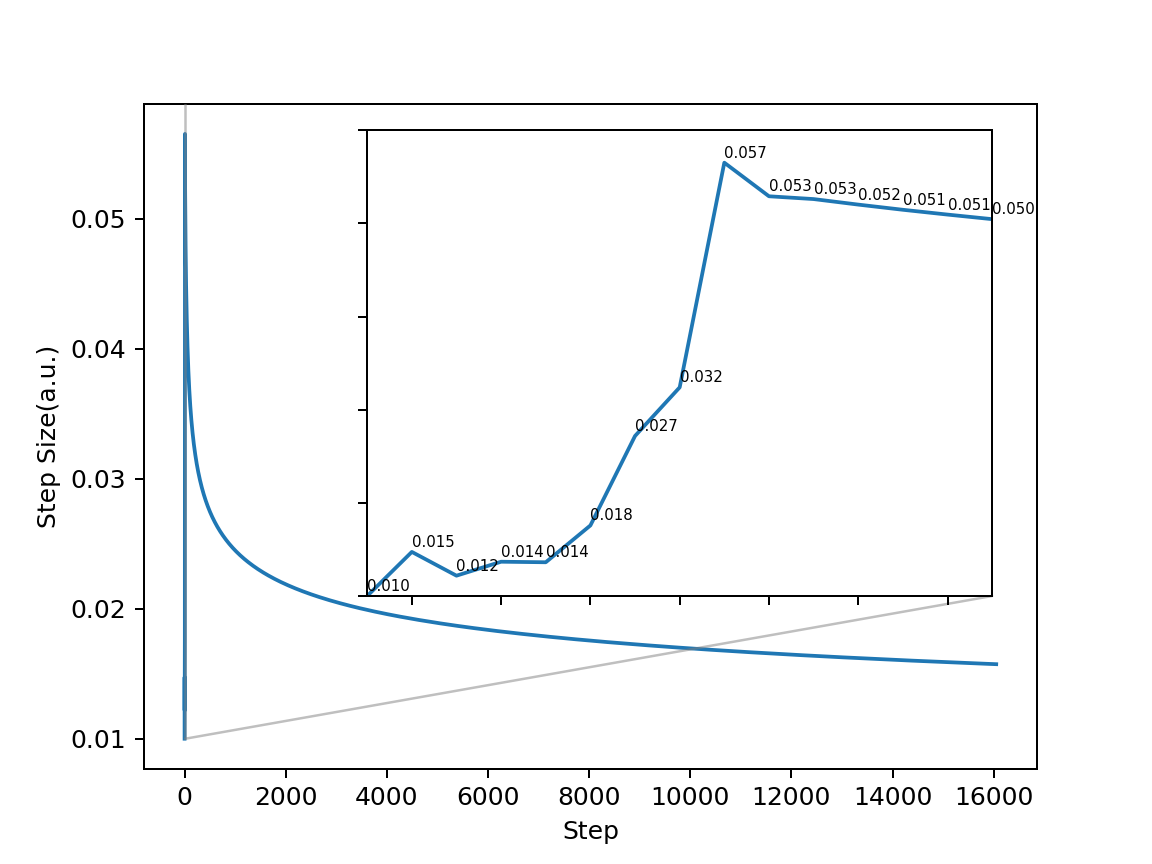
\includegraphics[angle=0, scale=0.3]{ch3/Figs/3-3_new.png}
    \caption{The adjusted step size at each time step in the RT-CCSD/cc-pVDZ
calculation for H$_2$O using the adaptive Cash-Karp integrator over 300 a.u.\
propagation. The first 15 time steps are zoomed in to focus on the detailed change.}
    \label{fig:ck-step}
\end{figure}

\begin{figure}
    \centering
    \begin{subfigure}{0.475\textwidth}
        \centering
        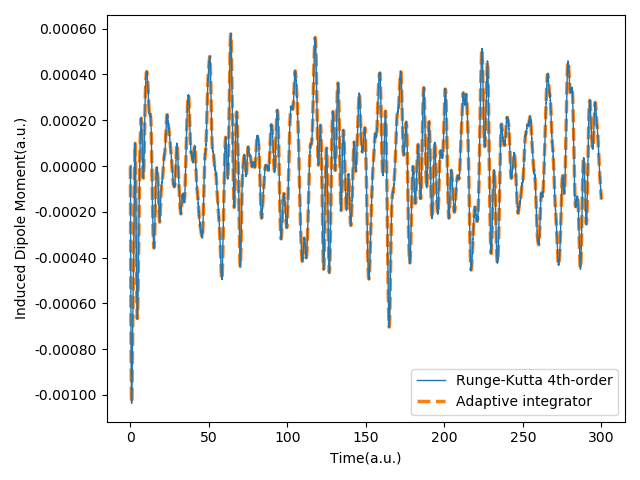
\includegraphics[width=\textwidth]{ch3/Figs/3-1.png}
    \end{subfigure}
    \hfill
    \begin{subfigure}{0.475\textwidth}
        \centering
        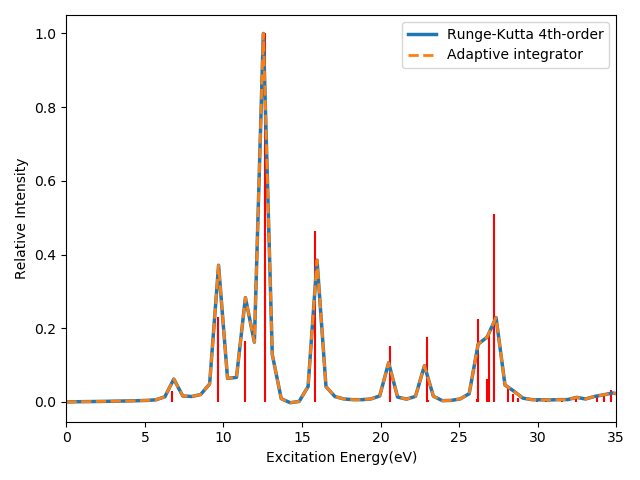
\includegraphics[width=\textwidth]{ch3/Figs/3-2.png}
    \end{subfigure}
    \caption{Comparison of the time-dependent induced dipole moment and the
corresponding linear absorption spectrum from the RT-CCSD/cc-pVDZ simulation of
H$_2$O using RK4 and CK integrators. EOM-CCSD/cc-pVDZ transition energies are
depicted as stick-spectra for reference.}
    \label{fig:ck-results}
\end{figure}

For strong external fields, the numerical stability of the propagation
becomes challenging because the wave function amplitudes fluctuate rapidly
leading to a large local error.  For example, Fig.~\ref{fig:t2-mag} depicts
the norm of the $\hat{T}_2$ amplitudes from an RT-CCSD/cc-pVDZ simulation
of our H$_2$O molecule at several different field strengths of the Gaussian
pulse in Eq.~(\ref{eq:field}) across a 1000 a.u.\ propagation using the RK4
integrator and a step size of $h = 10^{-2}$ a.u. On the scale of the
figure, the weaker fields of ${\cal E} = 0.01$ and $1.0$ a.u.\ induce
relatively small fluctuations in the amplitudes, while a $10.0$ a.u.\ field
yields much larger oscillations.  When the field strength is increased to
${\cal E} = 100.0$ a.u.\, the fluctuations are so great that the
propagation diverges. (This divergence affects both $\hat{T}$- and $\hat{\Lambda}$-amplitudes similarly.) In such cases, the TDSE is commonly referred to as a
``stiff equation'' in that the chosen step size must be extremely small to
maintain the stability of the propagation.  For our ${\cal E} = 100.0$
a.u.\ test case, we find that a step size of $h = 10^{-5}$ a.u.\ is
necessary to maintain the integrity of the simulation, which is clearly
impractical for realistic applications.

\begin{figure}
    \centering
    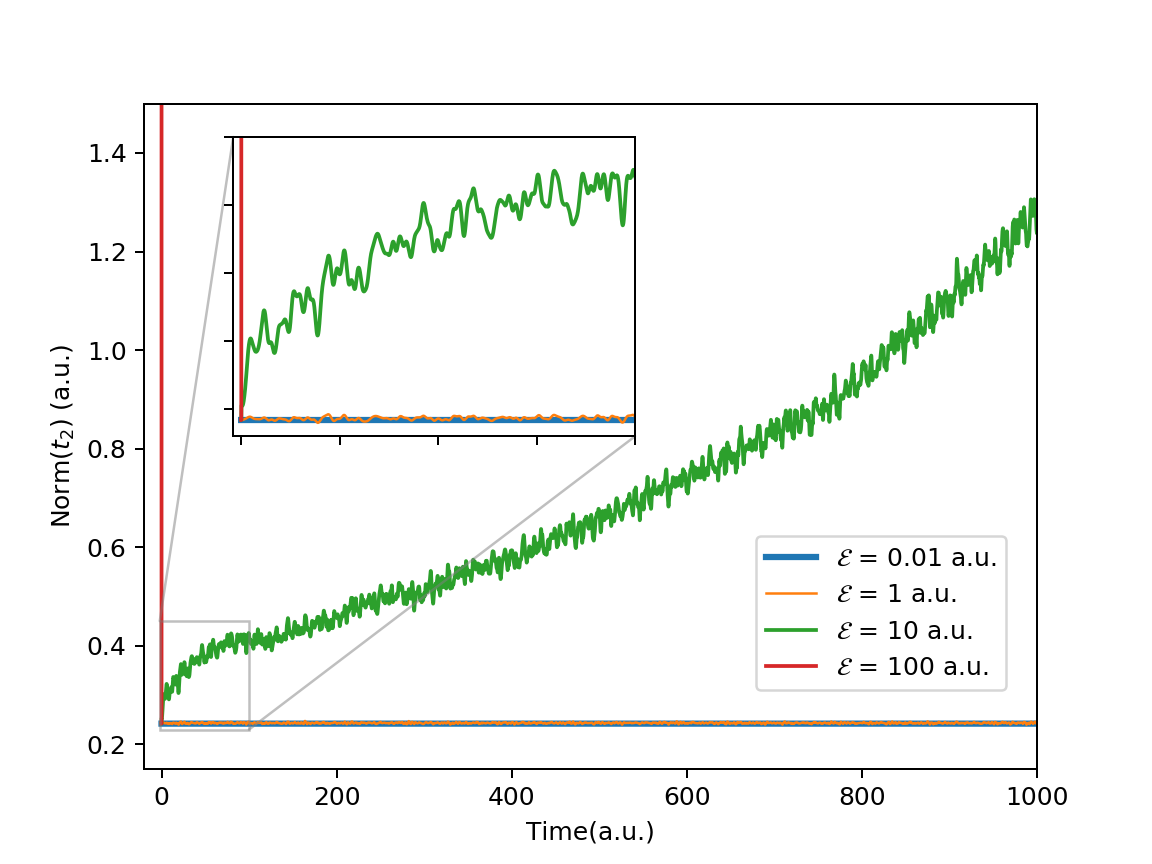
\includegraphics[angle=0, scale=0.3]{ch3/Figs/4-4.png}
    \caption{Comparison of the norm of $\hat{T}_2$ amplitudes during an
RT-CC/cc-pVDZ simulation for H$_2$O using a short Gaussian pulse and the RK4
integrator for different field strengths, ${\cal E}$.}
    \label{fig:t2-mag}
\end{figure}

For the strong-field simulation, it is noteworthy that the divergence
begins near the peak of the of the Gaussian pulse, suggesting that one
might need only decrease the step size while the field is on (the ``bumpy''
portion of the trajectory) and shift to larger values once the field has
decayed.  We therefore carried out a test simulation using $h_1 = 10^{-5}$
a.u.\ when the field is non-zero and $h_2 = 0.01$ a.u.\ otherwise.  The
overhead of this approach is obviously the number of additional residual
evaluations necessary during the pulse, $\frac{\Delta t}{h_{1}} -
\frac{\Delta t}{h_2}$, where $\Delta t$ is the duration of the
field.  The goal is to use steps from $t_{0}$ to $t_{f}$ to track the
interaction with the field precisely, while still minimizing the
computational cost for the overall propagation. 

In order to test this approach, we chose a very narrow Gaussian pulse with
$\nu=0.0005$ a.u.\ and $\sigma=0.0001$ a.u.\ according to the magnitude of
$h_{1}$, once again for an RT-CCSD/cc-pVDZ calculation for a single H$_2$O
molecule, but for a 1000 a.u.\ propagation.  For ${\cal E} = 100.0$ a.u.\
we found that the proposed mixed-step-size approach recovered a stable
propagation, as shown in Fig.~\ref{fig:ms-results}, whose upper-left-hand
plot depicts the norm of the $\hat{T}_2$ wave function parameters as a
function of time. The amplitude of the oscillation is clearly greater than
that induced by weaker fields, which is expected, but it still does not
diverge throughout the propagation. The corresponding absorption spectrum
in the lower-right-hand plot of Fig.~\ref{fig:ms-results} is nearly the
same as that produced by a weaker field in Fig.~\ref{fig:ck-results}, apart
from some additional noise in the low-frequency regime.

\begin{figure}
    \centering
    \begin{subfigure}{0.475\textwidth}
        \centering
        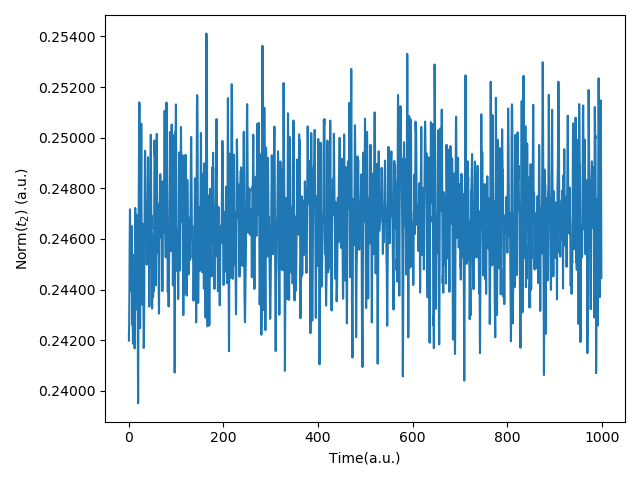
\includegraphics[width=\textwidth]{ch3/Figs/4-5.png}
    \end{subfigure}
    \hfill
    \begin{subfigure}{0.475\textwidth}
        \centering
        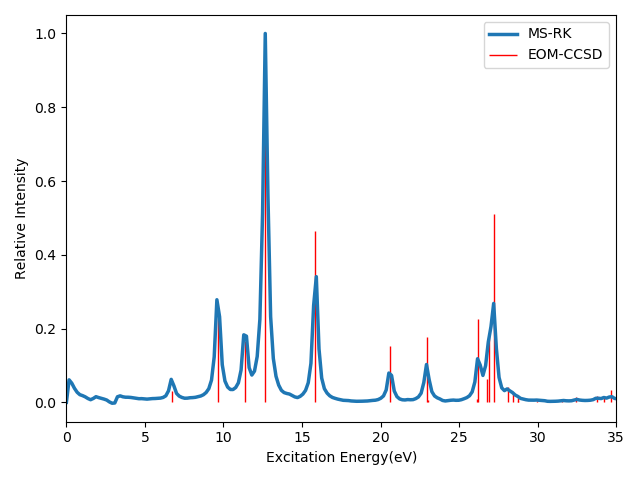
\includegraphics[width=\textwidth]{ch3/Figs/4-3.png}
    \end{subfigure}
    \\
    \begin{subfigure}{0.475\textwidth}
        \centering
        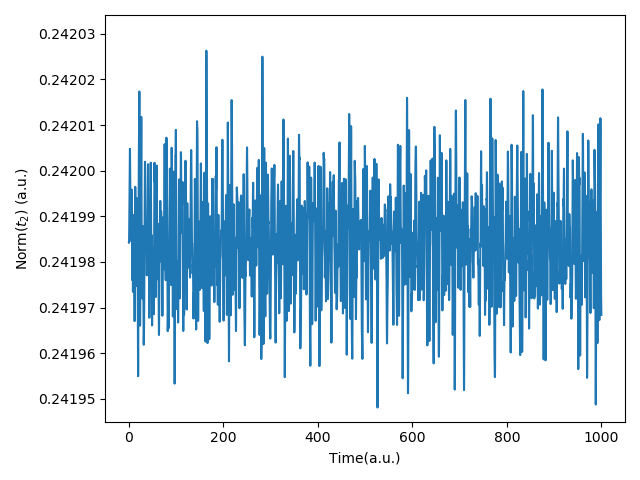
\includegraphics[width=\textwidth]{ch3/Figs/4-6.png}
    \end{subfigure}
    \hfill
    \begin{subfigure}{0.475\textwidth}
        \centering
        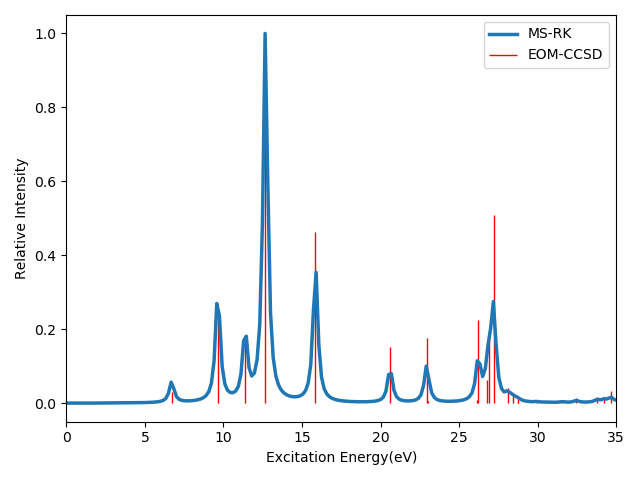
\includegraphics[width=\textwidth]{ch3/Figs/4-7.png}
    \end{subfigure}
    \\
    \begin{subfigure}{0.475\textwidth}
        \centering
        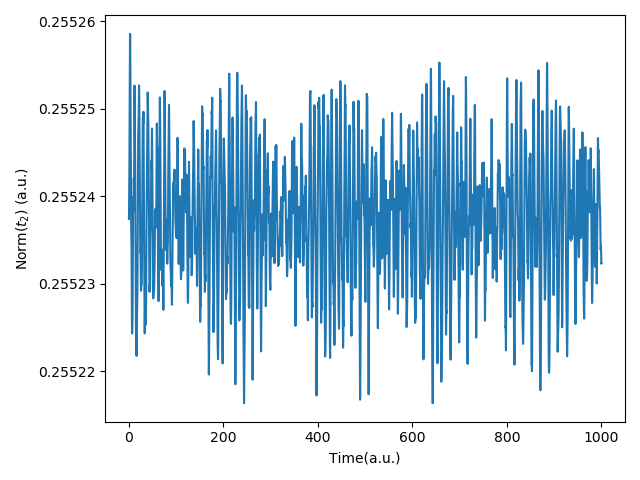
\includegraphics[width=\textwidth]{ch3/Figs/4-8.png}
    \end{subfigure}
    \hfill
    \begin{subfigure}{0.475\textwidth}
        \centering
        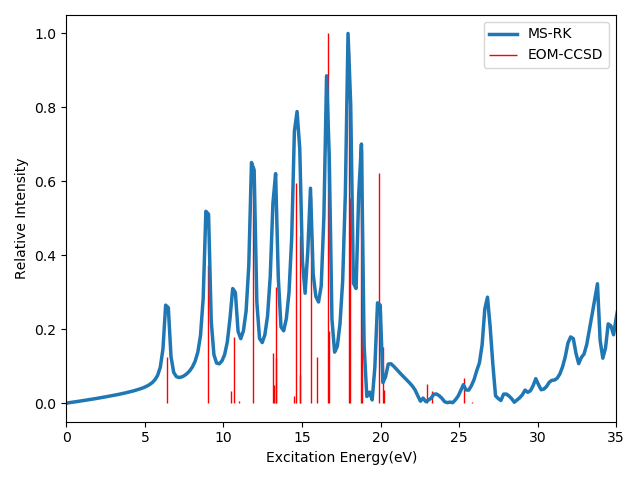
\includegraphics[width=\textwidth]{ch3/Figs/4-9.png}
    \end{subfigure}

    \caption{A $t=1000$ a.u.\ simulation of H$_2$O in the presence of a
    strong ${\cal E} = 100.0$ a.u.\ field with a width of $10^{-4}$ a.u.\
    (upper plot) and $10^{-6}$ a.u.\ (middle plot) at the RT-CCSD/cc-pVDZ
    level of theory using a mixed time-step RK4 approach. The bottom plot differs only from the middle calculation in
    that the aug-cc-pVDZ basis set was used, thus demonstrating that diffuse functions do not affect the numerical
    stability of this simulation.
    The norm of the
    $\hat{T}_2$ amplitudes in each case is depicted in the left-hand plots, and the
    absorption spectrum is shown on the right.}
\label{fig:ms-results}
\end{figure} 

The low-frequency noise disappears, however, if we also choose an even
narrower Gaussian pulse (so as to approximate a strong-field Dirac-delta
pulse) in conjunction with the mixed step-size approach described above.
To demonstrate this we chose parameters for the external field to be
$\cal{E} = 100$ a.u., $\sigma = 10^{-6}$ a.u. and $\nu = 5\times10^{-6}$
a.u.\ with a corresponding step size of $h_{1} =10^{-7}$ a.u.\ during the
pulse and the usual $h_{2} =0.01$ a.u.\ is used after field is off. (Note
that we carried out this calculation in single-precision, and thus
$10^{-7}$ is the smallest scale that can be selected to retain the required
accuracy.) As shown in the middle plots of Fig.~\ref{fig:ms-results}, the
even smaller step size (compared to $h=10^{-5}$ a.u.) gives rise to a more
stable propagation, and therefore, a higher-quality spectrum that avoids
the extra noise in the low-frequency range that appears in the upper-right
panel of Fig.~\ref{fig:ms-results}.  It should also be noted that the
overhead of this calculation is the same as the one with a wider Gaussian
pulse since the ratio $\frac{\Delta t}{h_{1}}$ is unchanged.  Furthermore,
while a mixed step-size approach will necessarily incur more overhead for
more comples field shapes, the stability offered by the algorithm may be
worth the additional expense. Finally we note that, while further testing is necessary to determine the robustness of this
approach across a range of molecular systems, the propagation is stable even for the same molecule and the aug-cc-pVDZ
basis set and with the oxygen $1s$-core electrons included in the correlation treatment. The simulation with aug-cc-pVDZ
basis set is shown in the lower plots of Fig.~\ref{fig:ms-results}.



